\documentclass[UTF8]{ctexart}
\usepackage{graphicx}
\usepackage{booktabs}
\usepackage{listings}
\usepackage{multirow}
\usepackage{mathtools}
\pagestyle{plain}
\begin{document}
\title{Solution}
\author{}
\date{\today}
\maketitle
\clearpage

\begin{center}
	\large{qiu}
\end{center}
\paragraph{} 如果将两个相邻数连边,那么它长这样。
\paragraph{} 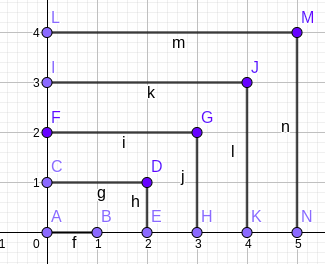
\includegraphics[]{1.png}
\paragraph{} 询问区间内(先容斥$(0,0)$为左下角的情况)一定是一些"-|"和一些"-"或"|"组成。
\paragraph{} 它们的和很好算。

\clearpage

\begin{center}
	\large{sky}
\end{center}
\paragraph{}很明显可以直接按pair排序,然后首先考虑$n\leq 100$,建立源点汇点,然后每个星辰拆成两个点
\begin{itemize}
\item 源点向所有入点连流量1费用0的边,汇点同理
\item 每个点$i$向所有排名小于等于其顺序的点$j$连一条流量1,费用为$-(b_i-b_j)$的边(自己也要连,因为流量可以不满)
\end{itemize}
\paragraph{}跑费用流即可,线段树优化建边可以跑到$n\leq 1000$
\paragraph{}接下来考虑模拟这个过程,新增的两个点分为两种情况,$i>j$和$i<j$(等号随意)
\begin{itemize}
\item $i>j$时,意味着我们只需要维护一个数据结构,使得可以找到最大的$i>j$边
\item $i<j$时,意味着如果存在此前一条边$x\rightarrow y$满足$x<i<j<y$,那么我们可以退掉$x\rightarrow y$的边连上$x\rightarrow i$,$j\rightarrow y$两条边
\end{itemize}
\paragraph{}找到最大的边可以拿线段树轻松维护,只需要支持单点修改,而另外一部分,我们可以考虑每选择一条边$i\rightarrow j$可以将$[i,j]$区间加一,这样如果一个区间内权值均为正数时可以退流
\paragraph{}所以此时再维护权值大于0的前缀最小值和后缀最大值,支持区间权值加减一即可。

\clearpage
\begin{center}
	\large{(dog)嫖怪}
\end{center}
\paragraph{子任务《一》$(10')$}
\paragraph{}爆搜,或者手动枚举都可以。
\paragraph{}这$10'$应该比前面的分都好拿吧。
\paragraph{}$100\%$的人都可以拿到这一档分。
\paragraph{子任务《二》$(30')$}
\paragraph{}这事实上是本题最有价值的一部分。
\paragraph{}先考虑小P的操作策略:每次必然会给非$1$的最小数加上$1$。
\paragraph{}因为如果不是给最小数加$1$,就有可能使这个数不再小于第$K$大而使操作无意义。同时,给$1$加上$1$也显然不优。
\paragraph{}再考虑嫖怪的操作策略,和小P的是完全一致的。所以为$1$的数可以直接特殊考虑。下面只讨论$\geq 2$的情况。
\paragraph{}现在我们手动模拟一个序列:$3 3 3 3 3$。
\paragraph{}我们会发现,小P一开始会使一个$3$变为$4$,然后失去一个$3$。
\paragraph{}继续模拟:令最小的数为$A_i$,个数为$a_i$,若干次操作后最小的数就会变为$A_i+1$,并且给它的个数加上$\frac{a_i}{2}$。
\paragraph{}另外一件事:当目前这个数恰好卡在第$K$大的时候,上面的结论还适用吗?
\paragraph{}显然是适用的。
\paragraph{}由于$A_i$只有$1$类,模拟这个过程即可。
\paragraph{子任务《三》$(10')$}
\paragraph{}我们现在考虑如何求出最小值。
\paragraph{}用$f_i$表示最小值为$i$时,有多少个为$i$的数。
\paragraph{}我们就有:$f_i=\frac{f_{i-1}}{2}+a_i$。
\paragraph{}而我们需要的是,消失的数第一次$\geq K$时的最小值。
\paragraph{}知道了之后,倒推到$= K$的情况也很简单了。
\paragraph{}还要考虑如何求出答案。
\paragraph{}小P按照上述策略操作后,显然每次操作就都有意义了。令初始局面为序列${a_i}$,终止局面为序列${b_i}$。答案就会是$\sum i*a_i-\sum i*b_i$。
\paragraph{子任务《四》$(50')$}
\paragraph{}我们现在考虑如何快速计算。
\paragraph{}上面那个东西显然是可以二分的。那么我们现在需要快速求出${f_i}$。
\paragraph{}简单推导可知$f_i=\frac{\sum {j=2}^{i-1} a_j*2^j }{2^i} + a_i$。
\paragraph{}你需要维护一个东西:$\frac{\sum {j=l}^{r} a_j*2^j }{2^r}$,这个放线段树上简单维护即可。
\paragraph{}那这道水题就做完了。
\end{document}